\section{Descrizione delle classi}
\subsection{Gerarchia degli utenti}

\begin{figure}[h]
  \caption{Struttura logica della gerarchia degli utenti}
  \centering
  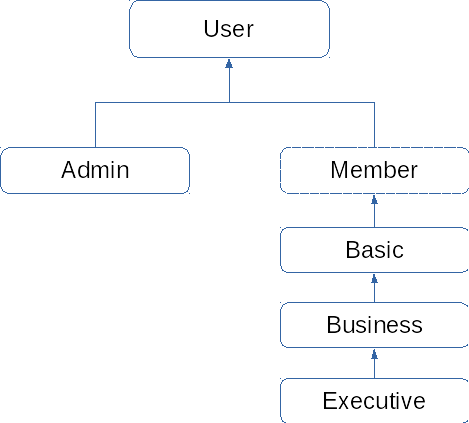
\includegraphics[width=8cm,height=8cm,keepaspectratio]{res/userclass}
\end{figure}

Alla base di tutta la gerarchia degli utenti � presente la classe \textit{Users}.
Questa \`e una classe virtuale, che contiene informazione di base,
come il tipo di account in uso, il Database a cui appartiene e la sua
validit\`a. Dato che logicamente non ha senso che esista un User, esso non
� istanziabile. \newline
Derivato a User c'\`e \textit{Admin}, che � una classe istanziabile e concreta.
Essa implementa le funzionalit\`a dell'amministratore, come il metodo
di ricerca, il cambiamento di tipo di un Membro, la sua aggiunta e la sua
cancellazione. \newline

Derivata da User c'\`e anche la classe \textit{Member}, virtuale pura.
Essa pone le basi per tutte le tipologie di iscritti a LinQedIn. Qui �
presente il metodo search da implementare per ogni classe derivata. Member
implementa gi� la scrittura e la lettura delle informazioni dal database
xml per ogni tipologia di iscritto. Basic, Business, Executive sono classi
derivate che implementano la ricerca sul Database.

\subsubsection{Classi contenute in Member}

Member contiene diverse classi, \textit{Profile} e \textit{Friendships} a
loro volta formate da pi\`u classi o derivate da altre.

\paragraph*{Profile} \`e una classe che contiene le informazioni
personali e la carriera dell'iscritto, ingloba tramite una relazione
\textit{has-a} le classi \textit{Personal} ed \textit{Experiences}. \newline
Personal contiene a sua volta \textit{Bio, Hobby, Interests}. \`E da
notare che \textit{Hobby, Interests} e \textit{Experiences} derivano da
classi contenitori. Questa scelta di creare dei wrapper \`e dovuta alla
maggiore estendibilit\`a del codice: se un domani si volesse cambiare
contenitore, le modifiche andrebbero eseguite solo in quelle classi.

\paragraph*{Friendships} deriva da un contanier \textit{vector} e si occupa
di salvare le amicizie di ogni Membro. L'amicizia viene salvata tramite il
nickName, che \`e univoco per tutto il Database.

\subsection{Gerarchia degli SmartPointer}

\begin{figure}[h]
  \caption{Struttura logica della gerarchia dei puntatori smart}
  \centering
  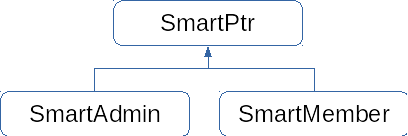
\includegraphics[width=8cm,height=8cm,keepaspectratio]{res/smartptrclass}
\end{figure}

Nonostante la gestione della memoria condivisa non sia stato un problema
data la natura implementativa del progetto, \`e stato deciso comunque
di utilizzare puntatori smart. SmartPtr \`e una classe base con il
costruttore dichiarato protected, questo per impedirne una sua
istanziazione tranne che per le classi derivate da essa: avere una classe
base comune a tutti i smartPtr permette di aggiungere funzionalit\`a a
tutte le classi derivate, e di introdurre metodi virtuali o puri.
\textit{SmartAdmin} e \textit{SmartMember} gestiscono la condivisione
in memoria rispettivamente di Admin e Member, utilizzando il reference
counting.

\subsection{Gerarchia della gestione degli User}

\begin{figure}[h]
  \caption{Struttura logica della gerarchia per la gestione degli User}
  \centering
  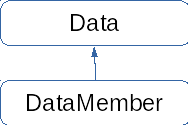
\includegraphics[width=3cm,height=3cm,keepaspectratio]{res/dataclass}
\end{figure}

Come scelta progettuale, si \`e deciso di non tenere la lista degli utenti
direttamente sul Database, ma di creare una gerarchia di classi per la
gestione di essi che poi verranno gestite a loro volta dal Database.
Questo permette una pi\`u facile gestione degli utenti (attualmente solo
Membri, ma potrebbero esserci altre tipologie).
La gerarchia ricalca la stessa struttura data per gli smart pointer e per
gli user.

\newpage %non ci sta in quella prima

\subsection{Database}

\begin{figure}[h]
  \caption{Gerachia del Database}
  \centering
  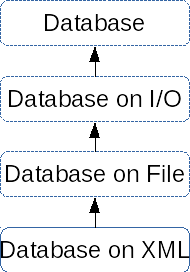
\includegraphics[width=5cm,height=5cm,keepaspectratio]{res/dbclass}
\end{figure}

Il Database \`e stato strutturato in maniera tale da rendere possibile la
scrittura della base di dati in diversi formati o in diversi device,
questo grazie alla derivazione da Database, classe virtuale pura in cui
vengono implementati solamente i metodi di ricerca (\textit{select})
sull'oggetto \textit{DataMember}, che si occupa come descritto prima
di mantenere in memoria gli iscritti al servizio. Per questo progetto \`e
stato deciso di salvare il database nel formato xml, ma grazie a questa
gerarchia \`e possibile implementare un diverso metodo di salvataggio.
Si noti come in DatabaseOnFile (nel codice viene chiamato \textit{DBonFile})
si ha una derivazione multipla: una dalla classe \textit{DBonIO}, l'altra
da \textit{QFile}; questo in quanto le classi derivate necessiteranno
delle funzioni di \textit{QFile} per riuscire a implementare le funzioni
pure di \textit{Database}.

\subsection{Interfaccia grafica}

\subsubsection{Pattern MVC}

Nella scrittura della GUI si \`e optato per l'uso del pattern MVC: si ha
quindi il \textit{Controller} che fa da ponte tra la \textit{View} e
il \textit{Model}, e si occupa di effettuare eventuali controlli di
consistenza con i dati e di elaborare gli imput provenienti dalla
\textit{View} stessa.

\subsubsection{Idea e schema di funzionamento}

\begin{figure}[h]
  \caption{Schema di funzionamento della GUI}
  \centering
  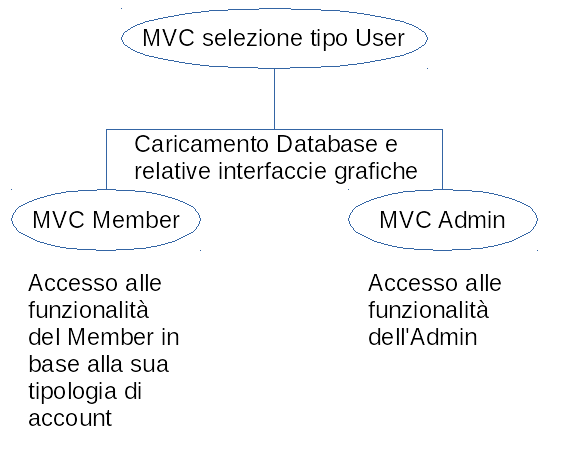
\includegraphics[width=8cm,height=8cm,keepaspectratio]{res/GUIscheme}
\end{figure}

La gestione dell'interfaccia grafica, basata sul pattern MVC, si prepone
di caricare in RAM solo la parte effettivamente utilizzata dal programma.
Dato che non \`e possibile cambiare utente dopo la selezione del tipo,
caricare in RAM anche l'altra parte di interfaccia grafica che non verr\`a
certamente usata sarebbe un inutile spreco di risorse. Quindi, il
\textit{MainWindowController} si occupa di far istanziare al
\textit{MainWindowModel} solamente la parte effettivamente utilizzata.

Per ogni funzionalit\`a \`e stato deciso di creare un proprio pattern MVC:
questo permette di isolare ogni parte in una propria finestra e
di rendere le modifiche a quella specifica sezione pi\`u semplici.

\newpage
\paragraph*{Gestione del Database} In base alla scelta del tipo di User,
viene creato un oggetto \textit{DBonXml}:
\begin{verbatim}
Database* db = new DBonXml(``database'');
\end{verbatim}
questo porta a una riduzione dell'estendibilit\`a del codice (se per esempio
si decidesse di apportare una modifica comune all'istanziazione del
database ci\`o dovrebbe essere ripetuto per tutti i controller che
istanziano il database), ma permette di apportare modifiche singole per
ogni controller che istanzia un Database.
